%-----------------------------------------
\chapter{Resultados usando el Modelo 1\\
(RNC desde cero)}

En esta sección se presentan los resultados obtenidos al usar el modelo 1 (\ver sección \ref{sec:modelo1}). Primero se presentan los resultados del modelo 1 usando la base de datos \textit{CharsPlateCol}, luego se muestran los resultados agregándole la base de datos \textit{Chars34} y finalmente se realiza una comparación de los dos resultados.

Inicialmente se muestran resultados en la clasificación de caracteres individuales. Es decir, la imagen de entrada a reconocer es un carácter que ha sido extraído previamente de una placa colombiana. Luego, se muestran resultados en la clasificación de toda la placa. Es decir, que la imagen de entrada al sistema corresponde a la parte frontal del automóvil donde se identifica la placa (ver sección \ref{sec:basedatos3}). De esta manera el sistema de reconocimiento completo consiste en una etapa de segmentación de cada caracter en la placa y luego una etapa de reconocimiento usando la RNC previamente entrenada.  

\section{Resultado usando la base de datos\\
\textit{CharsPlateCol}}

\subsection{Reconocimiento de caracteres segmentados}

Se presentan aquí los resultados en la clasificación de caracteres individuales después de ser segmentados desde las placas. Este primer resultado se muestra con el fin de observar si el sistema de reconocimiento falla por el entrenamiento de la RNC o por el proceso de segmentación.  

Las figura \ref{fig:Progreso del entrenamiento durante 200  ́época} muestra el progreso en el rendimiento tanto del conjunto entrenamiento como en el conjunto de validación durante las 200 épocas, usando solamente la base de datos \textit{CharsPlateCol}. La figura (a) muestra el progreso en la precisión y la figura (b) en la pérdida. Se observa un distanciamiento de las dos curvas aproximadamente a partir de las 75 épocas, lo que indica un entrenamiento no muy adecuado, ya que en ese momento no se ha logrado un buen rendimiento (alta precisión y baja perdida). 

\begin{figure}[H]
  \subfigure[]{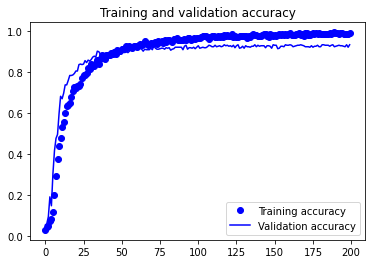
\includegraphics[width=0.5 \linewidth]{imagenes/MODEL_CARACTERES_SEGMENTADOS/ACCU.png}}
    \subfigure[]{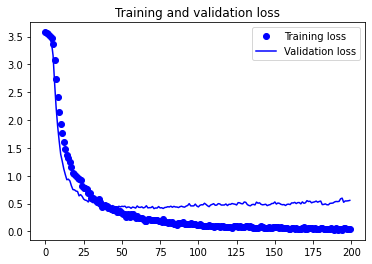
\includegraphics[width=0.5 \linewidth]{imagenes/MODEL_CARACTERES_SEGMENTADOS/LOSS.png}}
    \caption{Progreso del entrenamiento durante 200  ́épocas}
    \label{fig:Progreso del entrenamiento durante 200  ́época}  
\end{figure}


% Entrenamos a la CNN solo con caracteres segmentados y se logró un porcentaje de clasificación del 93\% en la evaluación del modelo. De las 519 imágenes del test, identificó con éxito 482, presentando dificultad en 37 de ellas. 



%En la muestra del resultado del test-modelo caracteres segmentados, podemos concluir que se presenta dificultad con caracteres con tienen algún tipo de irregularidad, ejemplo de eso, es la letra M, que es confundida por el modelo con una letra V, pero se puede comprender, ya que se evidencia que es un caracter incompleto, después de ser segmentado para crear la data de entrenamiento.  Las imágenes  (a) y (b) son una muestra de caracteres clasificados correcta e incorrectamente por el modelo.

\begin{comment}
\begin{figure}[H]
  \subfigure[]{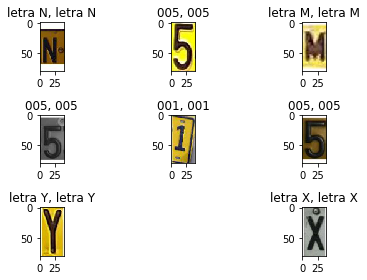
\includegraphics[width=0.4 \linewidth]{imagenes/MODEL_CARACTERES_SEGMENTADOS/CORREC_SEGMENTADAS.png}}
    \subfigure[]{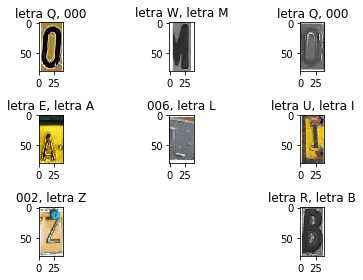
\includegraphics[width=0.4\linewidth]{imagenes/MODEL_CARACTERES_SEGMENTADOS/INCORREC_SEGMENTADA.png}}
    \caption{Resultado del test-modelo caracteres segmentados}
    \label{fig:(a) y (b) segmentada}  
\end{figure}

La figura \ref{fig:(a) y (b) segmentada} nos muestra en \textbf{(a)} 8 de las 482 caracteres clasificados correctamente en el test del modelo entrenado con la data segmentada y la imagen (b) es una muestra de 8 de los 37 caracteres clasificados incorrectamente por la red neuronal convolucional. 
\end{comment}

\subsection*{Rendimiento}

%En la figura \ref{fig:matrizconfusion1} se muestra la matriz de confusión. Podemos ver que el Modelo 1 presenta errores al momento de clasificar arrojando falso positivos y falsos negativos.

En la figura \ref{fig:matrizconfusion1} se muestra la Matriz de confusión obtenida de la evaluación del sistema usando 519 imágenes segmentadas de placas colombianas. Podemos observar en la diagonal principal el número de veces que una categoría Predicha por el modelo coincida con la Categoría verdadera. Mientras que un valor diferente de cero en las otras celdas nos indican los casos en que el modelo ha clasificado incorrectamente (Falsos Positivos y Falsos Negativos).

\begin{figure}[H]
\centering
  {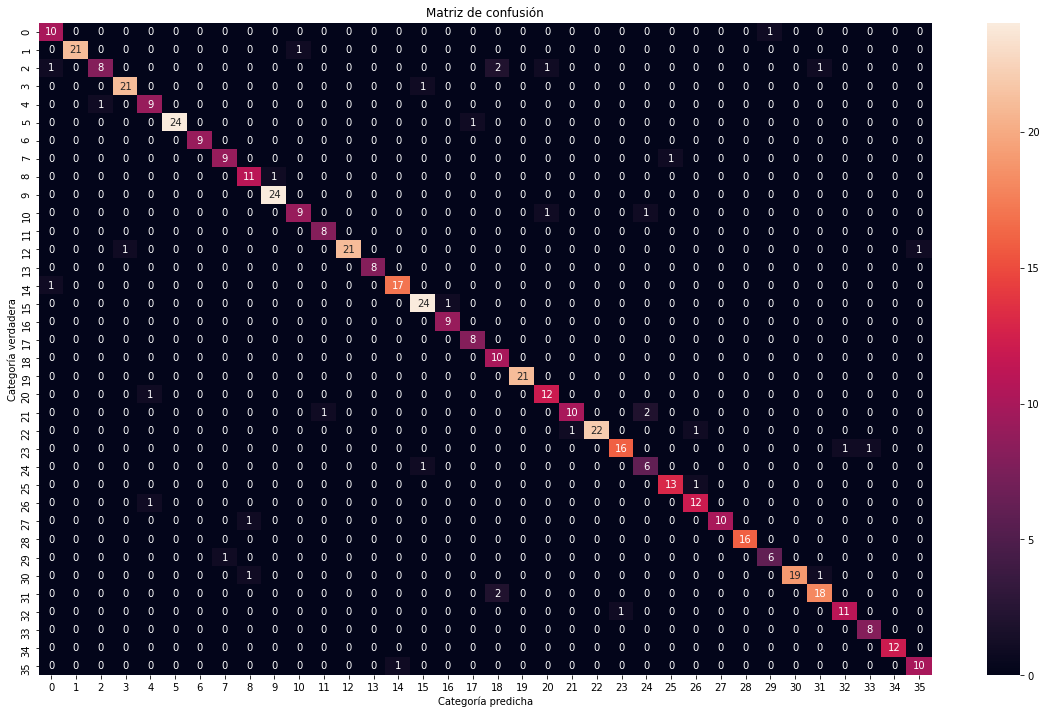
\includegraphics[width=0.7\linewidth]{imagenes/MODEL_CARACTERES_SEGMENTADOS/MATRIZ_CONFUSION.png}}
   \caption{Matriz de Confusión}
    \label{fig:matrizconfusion1}  
\end{figure}

La tabla \ref{table:Metricas segmentada} nos muestra los valores de las métricas (Precisión, Sensibilidad, valor-F1) calculados a partir de la matriz de confusión. Las métricas usadas para evaluar el Modelo 1 son el promedio ponderado de tales métricas, ya que la base de datos usada para el entrenamiento es desequilibrada (ver sección \ref{CharsPlateCol2.5k}). 

\begin{table}[H]
\begin{center}
\resizebox{0.4\textwidth}{!}{
\begin{tabular}{||c|c|c|c|c||}
\hline \hline
 Clases & Precisión &  Sensibilidad & Valor F &  Soporte\\
\hline \hline
     Clase 0 & 0.83 & 0.91 & 0.87 &  11\\\hline
     Clase 1 & 1.00 & 0.95 & 0.98 &  22\\\hline
     Clase 2 & 0.89 & 0.62 & 0.73 &  13\\\hline
     Clase 3 & 0.95 & 0.95 & 0.95 &  22\\\hline
     Clase 4 & 0.82 & 0.90 & 0.86 &  10\\\hline
     Clase 5 & 1.00 & 0.96 & 0.98 &  25\\\hline
     Clase 6 & 1.00 & 1.00 & 1.00 &   9\\\hline
     Clase 7 & 0.90 & 0.90 & 0.90 &  10\\\hline
     Clase 8 & 0.85 & 0.92 & 0.88 &  12\\\hline
     Clase 9 & 0.96 & 1.00 & 0.98 &  24\\\hline
    Clase 10 & 0.90 & 0.82 & 0.86 &  11\\\hline
    Clase 11 & 0.89 & 1.00 & 0.94 &   8\\\hline
    Clase 12 & 1.00 & 0.91 & 0.95 &  23\\\hline
    Clase 13 & 1.00 & 1.00 & 1.00 &   8\\\hline
    Clase 14 & 0.94 & 0.94 & 0.94 &  18\\\hline
    Clase 15 & 0.92 & 0.96 & 0.94 &  25\\\hline
    Clase 16 & 0.90 & 1.00 & 0.95 &   9\\\hline
    Clase 17 & 0.89 & 1.00 & 0.94 &   8\\\hline
    Clase 18 & 0.71 & 1.00 & 0.83 &  10\\\hline
    Clase 19 & 1.00 & 1.00 & 1.00 &  21\\\hline
    Clase 20 & 0.86 & 0.92 & 0.89 &  13\\\hline
    Clase 21 & 0.91 & 0.77 & 0.83 &  13\\\hline
    Clase 22 & 1.00 & 0.92 & 0.96 &  24\\\hline
    Clase 23 & 0.94 & 0.89 & 0.91 &  18\\\hline
    Clase 24 & 0.67 & 0.86 & 0.75 &   7\\\hline
    Clase 25 & 0.93 & 0.93 & 0.93 &  14\\\hline
    Clase 26 & 0.86 & 0.92 & 0.89 &  13\\\hline
    Clase 27 & 1.00 & 0.91 & 0.95 &  11\\\hline
    Clase 28 & 1.00 & 1.00 & 1.00 &  16\\\hline
    Clase 29 & 0.86 & 0.86 & 0.86 &   7\\\hline
    Clase 30 & 1.00 & 0.90 & 0.95 &  21\\\hline
    Clase 31 & 0.90 & 0.90 & 0.90 &  20\\\hline
    Clase 32 & 0.92 & 0.92 & 0.92 &  12\\\hline
    Clase 33 & 0.89 & 1.00 & 0.94 &   8\\\hline
    Clase 34 & 1.00 & 1.00 & 1.00 &  12\\\hline
    Clase 35 & 0.91 & 0.91 & 0.91 &  11\\\hline
\hline
    Exactitud &  & & 0.93  &  519\\\hline
   Macropromedio  &  0.92  &  0.93  &  0.92  &  519\\\hline
Promedio ponderado & \textcolor{red}{0.93}  &  \textcolor{red}{0.93}   & \textcolor{red}{0.93}  &  519\\
\hline
\hline
\end{tabular}
}
\caption{\label{table:Metricas segmentada}Métricas de rendimiento}
\end{center}
\end{table}

\subsection*{Análisis}
De acuerdo a la tabla \ref{table:Metricas segmentada} y la definición de las métricas consignadas en ella, se puede realizar el siguiente análisis:

Para evaluar el rendimiento de la red en la identificación de categorías por medio de imágenes que nunca fueron usadas para el entrenamiento utilizamos la métrica \textit{Valor-F} (ver sección: \ref{sec:metricas1}).

En la tabla \ref{table:Metricas segmentada} se muestran los valores del Valor-F obtenidos por cada una de las categorías obteniendo un Promedio Ponderado Valor-F de 0,93.\\ 

\begin{tcolorbox}
[colback=blue!5!white,colframe=blue!45!black,fonttitle=\bfseries,title=Conclusión]
   El modelo tiene un rendimiento del 93\% en reconocer categorías con imágenes que nunca fueron usadas para el entrenamiento de la red neuronal convolucional.
\end{tcolorbox}\\
\\
Ahora analizaremos que tanto el sistema logra reconocer un mismo caracter con características muy diferentes por el proceso de segmentación, deterioro de la placa o condiciones ambientales externas, teniendo en cuenta que este tipo de caracteres es muy común en este problema.

Así que Las imágenes de un mismo caracter pueden presentar característica diferentes por las razones descritas anteriormente. Todos estos factores pueden ocasionar que el sistema reporte falsos negativos.  

Para evaluar el rendimiento de la red en el reconocimiento de una misma categoría aunque sus imágenes presenten características diferentes usamos la métrica \emph{Sensibilidad} (ver sección: \ref{sec:metricas1}), ya que ésta sirve para evaluar qué tanto el sistema evita los falsos negativos.

En la tabla \ref{table:Metricas segmentada} se muestran los valores de la Sensibilidad obtenidos por cada una de las categorías obteniendo un Promedio Ponderado de la Sensibilidad de 0,93. \\
\begin{tcolorbox}
[colback=blue!5!white,colframe=blue!45!black,fonttitle=\bfseries,title=Conclusión]
   El modelo tiene un rendimiento del 93\% en reconocer un mismo caracter aunque se le presente en imágenes con características muy diferentes.
\end{tcolorbox}\\

Finalmente analizamos el resultado de la discriminación entre categorías diferentes con características similares. Es detallar que tanto el sistema logra aprender a discriminar entre dos caracateres como la \textbf{Letra Q/Letra O}, que presentan características muy similares.  Las imágenes de dos caracteres diferentes pueden presentar característica muy similares debido principalmente a su forma. Algunas veces, una la perspectiva o grado de inclinación del caracter puede generar una similitud con otro caracter, letra M/letra N. Todos estos factores pueden ocasionar que el sistema reporte falsos positivos.

Para evaluar el rendimiento de la red cuando se le presentan imágenes de distintos caracteres pero con características similares usamos la métrica Precisión (ver \ref{sec:metricas1}), ya que ésta sirve para evaluar qué tanto el modelo evita los falsos positivos.

En la tabla \ref{table:Metricas segmentada} se muestran los valores de la Precisión obtenidos por cada una de las categorías obteniendo un Promedio Ponderado de la Precisión de 0,93.\\

\begin{tcolorbox}
[colback=blue!5!white,colframe=blue!45!black,fonttitle=\bfseries,title=Conclusión]
   El modelo tiene un rendimiento del 93\% en discriminar entre categorías diferentes aunque se le presenten imágenes con características muy similares.
\end{tcolorbox}\\

%De acuerdo al Promedio Ponderado de la Precisión, el Modelo 1 detecta en un 93\% los casos positivos. De acuerdo al Promedio Ponderado de la 

%A pesar de tener una base de datos con pocas imágenes, obtuvimos buenos resultados en el promedio promedio Precisión (93\%). Aunque, para el uso que se le quiere dar al sistema de reconocimiento de placas (acceso y seguridad), este valor no es aceptable. 

%En cuanto a la exactitud del modelo, logramos un porcentaje del 93\% valor que tampoco es aceptable, nuestro objetivo es un valor mayor o igual al 99\%. 


%En cuanto a F1-score podemos concluir que nuestro modelo en algunas clases como la 2, ses confiable al momento de detectar la clase, a pesar de su dificultad al hacerlo, esto teniendo en cuenta que maneja una alta precisión y bajo recall, en el caso de la clase 24, es totalmente diferente, tenemos baja precisión y alto recall, lo que indica que el modelo detecta bien la clase, pero también incluye frecuentemente muestras de otras clases, lo mismo sucede con la clase 18. Debemos resaltar que tenemos clases que son manejadas perfectamente por el modelo, como la 6, 13, 19, 28 y 34.

\subsection{Reconocimiento de toda la placa}

Con el modelo entrenado para el reconocimiento de caracteres de placas Colombianas, colocamos a prueba todo el sistema, iniciando con el cargue de la imagen de entrada y todo el proceso de segmentación. (Ver sección \ref{fig:segmentación de caracteres}). La segmentación nos arroja los 6 caracteres que ser\'an la entrada uno por uno de la red neuronal convolucional, figura \ref{fig:segmentación de caracteres1}. El reconocimiento de los 6 caracteres hecho por la RNC se evidencia en la figura \ref{fig:Resultado del reconocimiento de caracteres charscolplate3.5k} 

\begin{figure}[H]
\centering
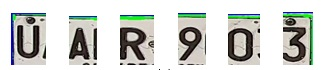
\includegraphics[width=0.7\linewidth]{imagenes/MODELO_4/segmentacion/segmentacion_figura2.jpg} \caption{segmentación de caracteres}
\label{fig:segmentación de caracteres1}
\end{figure}


\begin{figure}[H]
\centering
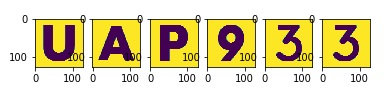
\includegraphics[width=0.9\linewidth]{imagenes/RESULTADOS/resultados_data_segmen.jpg} \caption{Resultado obtenido con una red neuronal convolucional para el reconocimiento de caracteres}
\label{fig:Resultado del reconocimiento de caracteres charscolplate3.5k}
\end{figure}

El modelo entrenado con la data segmentada, tiene inconvenientes en el reconocimiento de algunos caracteres, en este caso, se presenta dificultad al reconocer la letra \textbf{R} y el número \textbf{0}, que los confunde con la letra \textbf{P} y el número \textbf{3} respectivamente.

En general, el sistema de reconocimiento ha tenido mínimas fallas con letras que no tienen muchas imágenes en la data, como la letra H, que en pocos casos no logró reconocerla y la confundió con la letra T, igual sucede con la letra X cuando está incompleta después de la segmentación, la confunde con la letra K, pero ha sucedido con placas que tienen mucho brillo, aunque el problema radica en la segmentación, ya que tenemos placas desde diferentes perspectivas lo que implica un recorte diferente en cada caso y lleva al modelo a reconocer caracteres incompletos lo que hace que lo confunda con otro caracter. Los caracteres bien segmentados no han tenido inconvenientes al ser reconocidos, al igual que los caracteres incompletos, sino que en algunos casos tiene dificultad.

\section{Resultado usando la base de datos\\
\textit{CharsPlateCol} más la base de datos\\
\textit{{Chars34k}}}

\subsection{Reconocimiento de caracteres segmentados}
%La red neuronal ha sido entrenada nuevamente debido a la dificultad de clasificar algunos caracteres después del proceso de segmentación y entrenamiento con el modelo 1. En este ocasión hemos usado la data \textit{Chars34k} unida con la data \textit{charsplatecol2.5K}, para un total de 37.398 imágenes de 40 x 80 píxeles, que usaremos para el entrenamiento de la red neuronal convolucional bajo las mismas condiciones que el anterior entrenamiento, la diferencia será el uso de esta nueva data. La nueva data cuenta con un caracteres por clase en promedio 1000 imágenes. la letra \textbf{Q} es el caracter con el menor número, 886 y la letra \textbf{X} cuenta con exactamente 2065 imágenes. Ver cuadro \ref{table:imagenes por clase chars74k}\\


Los datos relacionados a continuación, son muy importantes para el entrenamiento de nuestra red convolucional, píxeles de las imágenes, cantidad de imágenes para el entrenamiento, validación y el test, el optimizador usado, entre otras. Tabla \ref{table:Hiperparametros Chars74K}

\begin{table}[H]
\begin{center}
\begin{tabular}{||c|c||}
\hline \hline
 Parámetros &  \\
\hline \hline
longitud-altura imagen & 80 x 40\\\hline
Imágenes de entrenamiento & 26253 \\ \hline
Imágenes de validación & 7405\\\hline
Imágenes de test & 3721\\\hline
INIT LR & 0.001 \\\hline
épocas & 200 \\\hline
batch size & 16\\ \hline
optimizador & SGD\\
\hline
\hline
\end{tabular}
\caption{\label{table:Hiperparametros Chars74K} Datos de entrenamiento}
\end{center}
\end{table}

%La red neuronal diseñada para el reconocimiento de caracteres de las placas colombianas de automóviles consta de 3 capas de convolución seguidas de una función de activación RELU y una capa maxpooling, luego tiene capas flatten, dense, dropout cerrando con una capa de activación softmax con 36 salidas, que nos indicará los porcentajes de clasificación obtenidos para cada clase. la estructura de esta red se muestra en la tabla \ref{table:estructura CNN}

%Cuando tenemos una imagen de entrada de 80x40 píxeles se le aplica una convolución cuyo filtro es 7x7 para generar 64 mapas de características de 74x34. A estos mapas se les aplica el filtro Max pooling de 2x2 y se obtienen mapas de características de 37x17. De igual forma hacemos con las siguientes convoluciones cuyos filtros son de 3x3, para obtener 128 mapas de 35x15, Luego del filtro Max pooling de 2x2, obtenemos mapas de 128 de 17x7. En la última convolución obtenemos 256 mapas de características de 15x5, que después del filtro Max pooling de 2x2 quedan de 7x2. Después de la etapa de extracción de características para el aprendizaje de la red, se realiza la clasificación a partir del flatten, dropout y la capa fully connected. Se finaliza con la función softmax, la cual asigna probabilidades a cada una de las clases al momento de realizar la clasificación. 

%La red neuronal entrenada recibe cada uno de los 6 caracteres segmentados y realiza su proceso de clasificación de acuerdo al entrenamiento realizado previamente. 

%En la primera etapa, se ha logrado segmentar en cada una de las placas, sus 6 caracteres con una efectividad de 98\%. En algunos casos el caracter queda al limite del recorte, y puede dificultar su correcta clasificación. El entrenamiento de la CNN se realizó en Colaboratory, un entorno gratuito de Jupyter Notebook que se ejecuta completamente en la nube. Entrenando la CNN solamente con caracteres de chars74K se obtuvo un porcentaje de clasificación de caracteres individuales que no superaba el 90\%. Pero, incluyendo para el entrenamiento las imágenes de caracteres segmentados de placas colombianas se logró un porcentaje del 99,49\% en la evaluación del modelo. De las 3.740 imágenes logró identificar correctamente 3.721, presentando dificultad en 19 de ellas. La figura \ref{fig:progreso del entrenamiento durante 200 épocas} muestra el progreso en el entrenamiento en cuanto a accuracy y loss respectivamente durante 200 épocas. 

Las figura \ref{fig:progreso del entrenamiento durante 200 épocas modelo2} muestra el progreso en el rendimiento tanto del conjunto entrenamiento como en el conjunto de validación durante las 200 épocas, usando la base de datos \textit{CharsPlateCol mas chars34k}. La figura (a) muestra el progreso en la precisión y la figura (b) en la pérdida. Se observa un buen comportamiento de la dos curvas que se ajustan a la curva del entrenamiento durante las 200 épocas, lo que indica un entrenamiento muy adecuado, ya que ha logrado un buen rendimiento (alta precisión y baja perdida). 

\begin{figure}[H]
  \subfigure[]{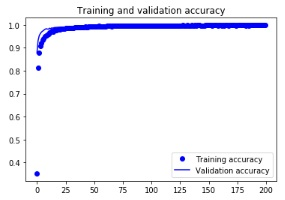
\includegraphics[width=0.5\linewidth]{imagenes/MODELO_4/ACCU_MOD_IV.jpg}}
    \subfigure[]{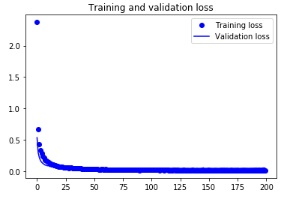
\includegraphics[width=0.5\linewidth]{imagenes/MODELO_4/LOSS_MOD_IV.jpg}}
    \caption{progreso del entrenamiento durante 200 épocas}
    \label{fig:progreso del entrenamiento durante 200 épocas modelo2}  
\end{figure}

\begin{comment}

En la muestra de los Resultados del test del modelo entrenado con la data \textit{Chars34K} más Data \textit{charsPlateCol2.5k}, nos enfocamos en los caracteres clasificados incorrectamente, concluyendo que algunos de esos caracteres tienen un nivel de dificultad bastante alto, como es el caso de la \textbf{letra J}, que además de tener un color gris está significativamente inclinada, la \textbf{letra o} está bastante pixelada, lo que indicaría que es la razón para ser confundida con una \textbf{letra p }

podemos concluir que se presenta dificultad con caracteres que tienen algún tipo de irregularidad, ejemplo de eso, es la letra M, que es confundida por el modelo con una letra V, pero se puede comprender, ya que se evidencia que es un caracter incompleto, después de ser segmentado para crear la data de entrenamiento.  En la figura \ref{fig:(a) y (b)} (a) y (b) son una muestra de caracteres clasificados correcta e incorrectamente por el modelo.

\begin{figure}[H]
  \subfigure[]{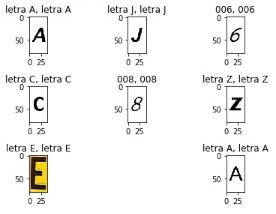
\includegraphics[width=0.5\linewidth]{imagenes/MODELO_4/CLASIF_MOD_IV.jpg}}
    \subfigure[]{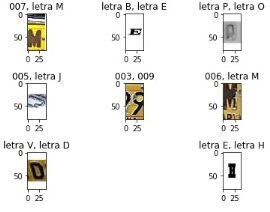
\includegraphics[width=0.5\linewidth]{imagenes/MODELO_4/NO_CLASIF_MOD_IV.jpg}}
    \caption{Resultados del test, modelo entrenado \textit{Chars34K} más Data \textit{CharsPlateCol2.5k}}
    \label{fig:(a) y (b)}  
\end{figure}

La figura \ref{fig:(a) y (b)} nos muestra en \textbf{(a)} 8 de las 3721 caracteres clasificados correctamente en el test del modelo entrenado con la data chars74K más data segmentada y la imagen (b) es una muestra de 8 de los 19 caracteres clasificados incorrectamente por la red neuronal convolucional. 
\end{comment}

\subsection*{Rendimiento}

En la figura \ref{fig:matriz de confusion chars74k más data} se muestra la Matriz de confusión obtenida de la evaluación del sistema usando 3740 imágenes segmentadas de placas colombianas y de la base de datos \textit{chars34k} escogidas aleatoriamente. Podemos observar en la diagonal principal el número de veces que una categoría Predicha por el modelo coincida con la Categoría verdadera. Mientras que un valor diferente de cero en las otras celdas nos indican los casos en que el modelo ha clasificado incorrectamente (Falsos Positivos y Falsos Negativos).

\begin{figure}[H]
\centering
  {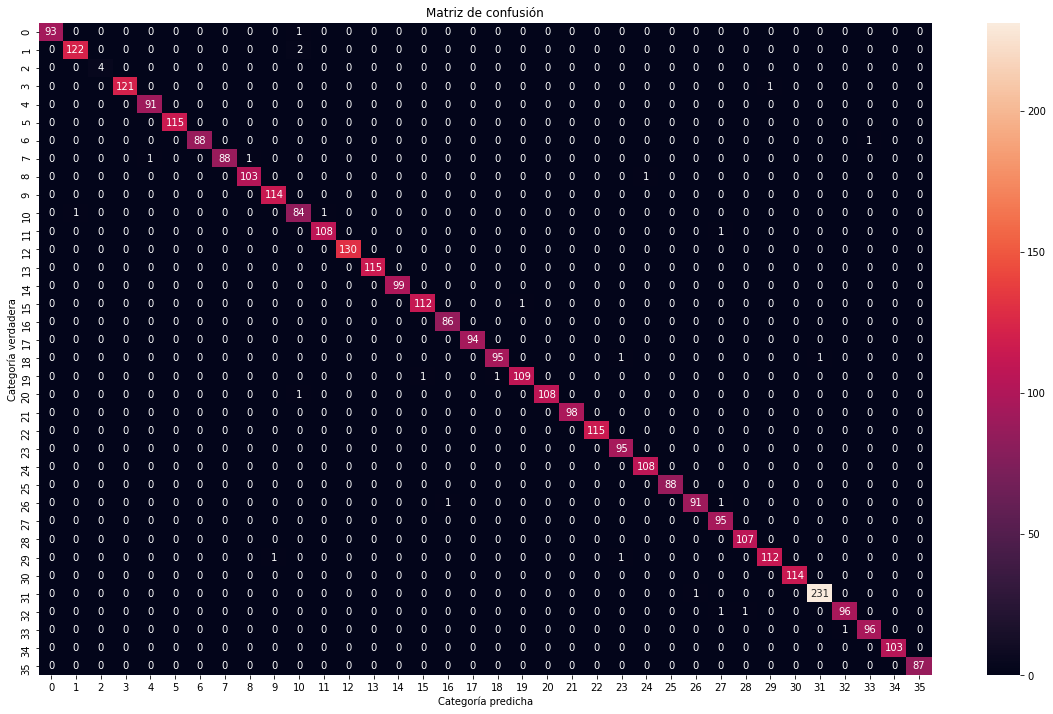
\includegraphics[width=0.5\linewidth]{imagenes/MODELO_4/matriz_de_confusion.png}}
  \caption{Matriz de confusión modelo Chars74K más Data Segmentada}
   \label{fig:matriz de confusion chars74k más data}  
\end{figure}

La tabla \ref{table:Metricas chars74k más data} muestra los valores de las métricas utilizadas para evaluar el rendimiento del modelo. En general, podemos observar que las métricas del modelo son muy buenas ya que se logra una  Exactitud del 99,49\%; un valor muy próximo al 100\% que nos indica  la cantidad de predicciones positivas que fueron correctas. 

Para evaluar el rendimiento general de la red en la identificación de categorías por medio de imágenes que nunca fueron usadas para el entrenamiento utilizamos la métrica \textit{Valor-F} (ver sección: \ref{sec:metricas1}).

El PP Valor-F es de 0,9949,  en este caso podemos afirmar que nuestro modelo maneja perfectamente cada clase, ya que tenemos valores de alta precisión y alta Sensibilidad. Además, podemos observar que tenemos 13 clases reconocidas 100\% por nuestro modelo.\\

 \begin{tcolorbox}
[colback=blue!5!white,colframe=blue!45!black,fonttitle=\bfseries,title=Conclusión]
   El modelo tiene un rendimiento del 99,49\% en reconocer categorías con imágenes que nunca fueron usadas para el entrenamiento de la red neuronal convolucional.
\end{tcolorbox}\\

\newpage

\begin{table}[H]
\begin{center}
\resizebox{.5\textwidth}{!}{
\begin{tabular}{||c|c|c|c|c||}
\hline \hline
 Clases & Precisión  &  Sensibilidad & Valor F  & Soporte\\
\hline \hline
Clase 0  &   1.0000 &   0.9894 &   0.9947  &   94\\\hline
Clase 1  &   0.9919 &   0.9839 &   0.9879  &   124\\\hline
Clase 2  &   1.0000 &   1.0000 &   1.0000  &   4\\\hline
Clase 3  &   1.0000 &   0.9918 &   0.9959  &   122\\\hline
Clase 4  &   0.9891 &   1.0000 &   0.9945  &   91\\\hline
Clase 5  &   1.0000 &   1.0000 &   1.0000  &   115\\\hline
Clase 6  &   1.0000 &   0.9888 &   0.9944  &   89\\\hline
Clase 7  &   1.0000 &   0.9778 &   0.9888  &   90\\\hline
Clase 8  &   0.9904 &   0.9904 &   0.9904  &   104\\\hline
Clase 9  &   0.9913 &   1.0000 &   0.9956  &   114\\\hline
Clase 10  &   0.9545 &   0.9767 &   0.9655  &   86\\\hline
Clase 11  &   0.9908 &   0.9908 &   0.9908  &   109\\\hline
Clase 12  &   1.0000 &   1.0000 &   1.0000  &   130\\\hline
Clase 13  &   1.0000 &   1.0000 &   1.0000  &   115\\\hline
Clase 14  &   1.0000 &   1.0000 &   1.0000  &   99\\\hline
Clase 15  &   0.9912 &   0.9912 &   0.9912  &   113\\\hline
Clase 16  &   0.9885 &   1.0000 &   0.9942  &   86\\\hline
Clase 17  &   1.0000 &   1.0000 &   1.0000  &   94\\\hline
Clase 18  &   0.9896 &   0.9794 &   0.9845  &   97\\\hline
Clase 19  &   0.9909 &   0.9820 &   0.9864  &   111\\\hline
Clase 20  &   1.0000 &   0.9908 &   0.9954  &   109\\\hline
Clase 21  &   1.0000 &   1.0000 &   1.0000  &   98\\\hline
Clase 22  &   1.0000 &   1.0000 &   1.0000  &   115\\\hline
Clase 23  &   0.9794 &  1.0000  &  0.9896   &   95\\\hline
Clase 24  &   0.9908 &   1.0000 &   0.9954  &   108\\\hline
Clase 25  &   1.0000 &   1.0000 &   1.0000  &   88\\\hline
Clase 26  &   0.9891 &   0.9785 &   0.9838  &   93\\\hline
Clase 27  &   0.9694 &   1.0000 &   0.9845  &   95\\\hline
Clase 28  &   0.9907 &   1.0000 &   0.9953  &   107\\\hline
Clase 29  &   0.9912 &   0.9825 &   0.9868  &   114\\\hline
Clase 30  &   1.0000 &   1.0000 &   1.0000  &   114\\\hline
Clase 31  &   0.9957 &   0.9957 &   0.9957  &   232\\\hline
Clase 32  &   0.9897 &   0.9796 &   0.9846  &   98\\\hline
Clase 33  &   0.9897 &   0.9897 &   0.9897  &   97\\\hline
Clase 34  &   1.0000 &   1.0000 &   1.0000  &   103\\\hline
Clase 35  &   1.0000 &   1.0000 &   1.0000  &   87\\\hline
\hline
Exactitud  &  &  & 0.9949  &   3740\\\hline
Macropromedio &   0.9932 &   0.9933 &   0.9949  &   3740\\\hline
Promedio Ponderado  & \textcolor{red}{0.9934} &   \textcolor{red}{0.9933} &  \textcolor{red}{ 0.9949}  &   3740\\\hline
\hline
\end{tabular}
}
\caption{\label{table:Metricas chars74k más data}Métricas entrenamiento Chars74K más Data Segmentada}
\end{center}
\end{table}



%En la tabla \ref{table:Metricas chars74k más data} se muestran los valores del Valor-F obtenidos por cada una de las categorías obteniendo un Promedio Ponderado Valor-F de 0,9949. 

   % \begin{tcolorbox}
%[colback=blue!5!white,colframe=blue!45!black,fonttitle=\bfseries,title=Conclusión 1]
 %  El modelo tiene un rendimiento del 99,49\% en reconocer categorías con imágenes que nunca fueron usadas para el entrenamiento de la red neuronal convolucional.
%\end{tcolorbox}\\
%\\
Ahora analizaremos que tanto el sistema logra reconocer un mismo caracter con características muy diferentes por el proceso de segmentación, deterioro de la placa o condiciones ambientales externas, teniendo en cuenta que este tipo de caracteres es muy común en este problema. Así que, las imágenes de un mismo caracter pueden presentar característica diferentes por las razones descritas anteriormente. Todos estos factores pueden ocasionar que el sistema reporte falsos negativos. Para evaluar el rendimiento de la red en el reconocimiento de una misma categoría aunque sus imágenes presenten características diferentes usamos la métrica \emph{Sensibilidad} (ver sección: \ref{sec:metricas1}), ya que ésta sirve para evaluar qué tanto el sistema evita los falsos negativos. 
En la tabla \ref{table:Metricas chars74k más data} se muestran los valores de la Sensibilidad obtenidos por cada una de las categorías obteniendo un Promedio Ponderado de la Sensibilidad de 0,9933. \\

\begin{tcolorbox}
[colback=blue!5!white,colframe=blue!45!black,fonttitle=\bfseries,title=Conclusión]
   El modelo tiene un rendimiento del 99,33\% en reconocer un mismo caracter aunque se le presente en imágenes con características muy diferentes.
\end{tcolorbox}\\

Finalmente analizamos el resultado de la discriminación entre categorías diferentes con características similares. Es detallar que tanto el sistema logra aprender a discriminar entre dos caracteres como la \textbf{Letra Q/Letra O}, que presentan características muy similares.  Las imágenes de dos caracteres diferentes pueden presentar característica muy similares debido principalmente a su forma. Algunas veces, una la perspectiva o grado de inclinación del caracter puede generar una similitud con otro caracter, letra M/letra N. Todos estos factores pueden ocasionar que el sistema reporte falsos positivos.

Para evaluar el rendimiento de la red cuando se le presentan imágenes de distintos caracteres pero con características similares usamos la métrica Precisión (ver \ref{sec:metricas1}), ya que ésta sirve para evaluar qué tanto el modelo evita los falsos positivos.

En la tabla \ref{table:Metricas chars74k más data} se muestran los valores de la Precisión obtenidos por cada una de las categorías obteniendo un Promedio Ponderado de la Precisión de 0,9934.\\

\begin{tcolorbox}
[colback=blue!5!white,colframe=blue!45!black,fonttitle=\bfseries,title=Conclusión 3]
   El modelo tiene un rendimiento del 99,34\% en discriminar entre categorías diferentes aunque se le presenten imágenes con características muy similares.
\end{tcolorbox}\\

\subsection{Reconocimiento de toda la placa}

Con el modelo entrenado para el reconocimiento de caracteres de placas Colombianas, colocamos a prueba todo el sistema. La entrada es toda la imagen del vehiculo con la placa para comenzar con el proceso de segmentación. (Ver sección \ref{fig:segmentación de caracteres}). La segmentación nos arroja los 6 caracteres que ser\'an la entrada uno por uno de la red neuronal convolucional, tal como se muestra en la figura \ref{fig:segmentación de caracteres} y el resultado del reconocimiento de los 6 caracteres, realizado por la RNC, se muestra en la figura \ref{fig:Resultado obtenido con una red neuronal convolucional para el reconocimiento de caracteres chars34k} 


\begin{figure}[H]
\centering
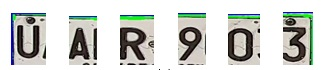
\includegraphics[width=0.7\linewidth]{imagenes/MODELO_4/segmentacion/segmentacion_figura2.jpg} \caption{segmentación de caracteres}
\label{fig:segmentación de caracteres}
\end{figure}

\begin{figure}[H]
\centering
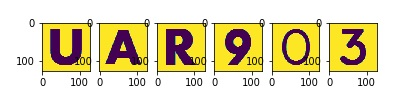
\includegraphics[width=0.9\linewidth]{imagenes/MODELO_4/segmentacion/resultado_carro4.jpg} \caption{Resultado obtenido con una red neuronal convolucional para el reconocimiento de caracteres}
\label{fig:Resultado obtenido con una red neuronal convolucional para el reconocimiento de caracteres chars34k}
\end{figure}

\begin{tcolorbox}
[colback=blue!5!white,colframe=blue!45!black,fonttitle=\bfseries,title=Conclusión]

Teniendo en cuenta el rendimiento de todo el sistema, podemos evidenciar la mejora al momento de reconocer los 6 caracteres de la misma placa , haciendo uso en este caso de la red neuronal convolucional entrenada con la Data \textit{Chars34K} más Data \textit{charsPlateCol}, donde logra reconocer el 100\% de los caracteres. Si el análisis lo relacionamos con las métricas, la exactitud en el modelo de la data \textit{charsPlateCol} es de 0.93 y en el modelo que se complementa con la data \textit{Chars34K} obtiene una exactitud del 0.9949. Debemos tener presente que esta Red neuronal convolucional para la clasificación, fue construida desde cero, iniciando sus entrenamientos con otros datas públicas(perros, gatos, leones) y finalizando con las data de caracteres, así mismo se diseño y construyó la base de datos para caracteres segmentados, que posteriormente fue usada para el entrenamiento en las dos RNC propuestas anteriormente.


\begin{table}[H]
\begin{center}
\resizebox{.9\textwidth}{!}{
\begin{tabular}{||c||c||c||}
\hline \hline
 \textbf{Métrica} & \textbf{Modelo data \textit{charsPlateCol2.5k}} & \textbf{\textit{Chars34K} más Data \textit{charsPlateCol2.5k}}\\
 \hline \hline
 PP. Valor-F & 0.93 & \colorbox{yellow}{0.9949}\\
 \hline
 Pérdida & 0.3113 & \colorbox{yellow}{0.0961}\\
 \hline \hline
 \end{tabular}
 }
 \caption{\label{blobs}Resultados por entrenamiento.}
\label{tabla:resultados metricas}
\end{center}
\end{table}
\end{tcolorbox}
\\

\begin{tcolorbox}
[colback=green!5!white,colframe=green!45!black,fonttitle=\bfseries,title=Contribución]

Esta primera parte de los resultados fue presentada en XVI Encuentro Nacional de Óptica VII y Conferencia Andina y del Caribe en Óptica y sus Aplicaciones (ENO-CANCOA) llevada a cabo del 26 al 30 de noviembre del 2019 en la ciudad de Montería, Colombia (ver Apéndice B).

El artículo correspondiente con título: 
\emph{Automatic recognition of Colombian car license plates using convolutional neural networks and Chars74k database}, está publicado en la Revista \emph{Journal of Physics: Conference Series} \cite{Arroyo-Perez2020ColombianLearning} (Ver apéndice C)
\end{tcolorbox}
